\documentclass[10pt]{article}
\usepackage[%
left=0.984252in,%
right=0.787402in,%
top=0.787402in,%
bottom=0.787402in,%
paperheight=11in,%
paperwidth=8.5in%
]{geometry}%

\usepackage{xeCJK}
\usepackage{blindtext}
\usepackage[T1]{fontenc}
\usepackage{caption}
\usepackage{graphicx}
\usepackage{textcomp}
\usepackage{fancyhdr}
\usepackage{listings}

\pagestyle{fancy}
\fancyhf{}
\fancyhead[R]{\thepage}
\usepackage{float}
\usepackage{alltt}

\setCJKmainfont{AozoraMinchoRegular.ttf}
\setCJKsansfont{AozoraMincho-bold.ttf}


\setCJKmainfont{AozoraMinchoRegular.ttf}
\setCJKsansfont{AozoraMincho-bold.ttf}

\usepackage{indentfirst}

\title{2 部データ構造とアルゴリズムI レポート課題2}
\author{18NC021 }
\date{カトリ スザン}
\captionsetup[table]{name=表}
\captionsetup[figure]{name=図}

\begin{document}

\begin{titlepage}
	\maketitle
\end{titlepage}

\tableofcontents
\pagebreak

\section{課題1のプログラム}
課題2では課題1で作った以下のプログラムを使う。

\subsection{shohin.h}
\begin{lstlisting}[language=C]
    #ifndef C_ALGO_REPORT2_SHOHIN_H
    #define C_ALGO_REPORT2_SHOHIN_H
    
    #endif //C_ALGO_REPORT2_SHOHIN_H
    
    
    #define ZEI (1.08)
    typedef struct{
        char* name;
        int tanka;
        int sotozei;
    } SHOHIN;
    extern SHOHIN shohin[];
    void printshohin(SHOHIN s);
\end{lstlisting}

\subsection{shohin.c}
\begin{lstlisting}[language=C]
    #include <stdio.h>
    #include "shohin.h"
    
    SHOHIN shohin[] = {{"Apple",  150},
                       {"Orange", 100},
                       {"Banana", 200},
                       {"Book1",  500, 1},
                       {"",       0}};
    
    void printshohin(SHOHIN s) {
        printf("%s\t単価%d円(%s)", s.name, s.tanka, s.sotozei ? "外税" : "内税");
    }
\end{lstlisting}

\subsection{uriage.h}
\begin{lstlisting}[language=C]
    #ifndef C_ALGO_REPORT2_URIAGE_H
    #define C_ALGO_REPORT2_URIAGE_H
    
    #endif //C_ALGO_REPORT2_URIAGE_H
    
    typedef struct {
        int code;
        int num;
    }URIAGE;
    
    int printUriage(URIAGE* q);
    int printUriageArray(URIAGE q[]);
    int printUriageTrans(URIAGE **p);
\end{lstlisting}

\subsection{uriage.c}
\begin{lstlisting}[language=C]
    #include <stdio.h>
    #include "uriage.h"
    #include "shohin.h"
    
    int printUriage(URIAGE *p) {
    
        char *const product_name = shohin[p->code].name;
        const int item_price = shohin[p->code].tanka;
        const int tax = shohin[p->code].sotozei;
        const int total_sales = p->num;
        const int total_price =
                tax ? (item_price * total_sales) * ZEI : item_price * total_sales;
        printf("%s\t 単価%d円(%s)\t%d 個\t%d円 \n", product_name, item_price,
               tax ? "外税" : "内税", total_sales, total_price);
        return total_price;
    }
    
    int printUriageArray(URIAGE u[]) {
        int shokei = 0;
        for (int i = 0; u[i].code != -1; i++) {
            shokei += printUriage(&u[i]);
        }
        return shokei;
    }
    
    int printUriageTrans(URIAGE **u) {
        int sub_total = 0;
        int total = 0;
        for (int i = 0; u[i] != NULL; i++) {
            sub_total = printUriageArray(*(u + i));
            total += sub_total;
            printf("小計:\t\t\t\t\t%d円\n", sub_total);
            printf("------------------------------------\n");
        }
        printf("合計:\t\t%d円\n", total);
        return total;
    }
\end{lstlisting}
\pagebreak

\section{課題2}

\subsection{課題2-1}

\begin{itemize}
    \item 線形リストの内容を表示する関数 void printUriageList(URIAGELIST* l) を作成しなさい。
\end{itemize}
\subsubsection{uriagelist.h}
\begin{lstlisting}[language=C]
    #ifndef C_ALGO_REPORT2_URIAGELIST_H
    #define C_ALGO_REPORT2_URIAGELIST_H
    #endif //C_ALGO_REPORT2_URIAGELIST_H
    
    typedef struct uriagelist {
        struct uriagelist* next;
        URIAGE *uriage;
    } URIAGELIST;
    
    void printUriageList(URIAGELIST* l);
\end{lstlisting}

\subsubsection{uriagelist.c}
\begin{lstlisting}[language=C]
    #include <stdio.h>
    #include <stdlib.h>
    #include "uriage.h"
    #include "shohin.h"
    #include "uriagelist.h"
    
    void printUriageList(URIAGELIST *l) {
        if (l->uriage == NULL) {
            return;
        }
        while (l->next != NULL) {
            // 課題1のuriage.cで定義されているprintUriage関数を使っている。
            printUriage(l->uriage);
            l = l->next;
        }
    }
\end{lstlisting}

\subsubsection{テストプログラム2-1}
\begin{lstlisting}[language=C]
    #include <stdio.h>
    #include <stdlib.h>
    #include "shohin.h"
    #include "uriage.h"
    #include "uriagelist.h"
    int main(void){
      URIAGE u1={1,2};
      URIAGE u2={2,3};
      URIAGE u3={3,4};
      URIAGELIST l0={NULL};
      URIAGELIST l1={&l0,&u1};
      URIAGELIST l2={&l1,&u2};
      URIAGELIST l3={&l2,&u3};
      printf("-----\n");
      printUriageList(&l0);
      printf("-----\n");
      printUriageList(&l1);
      printf("-----\n");
      printUriageList(&l2);
      printf("-----\n");
      printUriageList(&l3);
      return 0;
    }
\end{lstlisting}

\subsubsection{実行結果}
\begin{figure}[H]
	\centering
	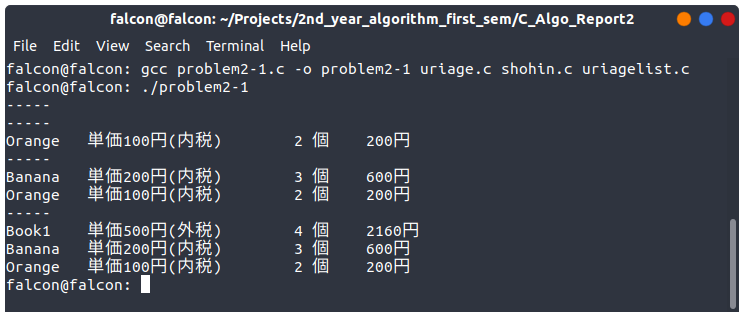
\includegraphics[width=0.8\textwidth]{problem2-1.png}
	\caption{課題2-1実行結果}
\end{figure}

\subsubsection{プログラムの解説}
\begin{itemize}
    \item このプログラムでは課題1で定義した、URIAGE型、SHOHIN型とprintUriage関数を使っている。
\end{itemize}
線形リストを構成する,一つひとつのノードは,データと次のノードを指すポインタとでできていて、このプログラムでは複数個のものが一つにまとまったものを構成するため構造体( : URIAGELIST)をつかっている。URIAGELIST構造体は次のノードのポインターとURIAGE型のポインター(uriage)から構成されている。URIAGELISTはuriagelist.hヘッダーファイルで定義している。 \\

uriagelist.cのprintUriageListはURIAGELIST型のポインター(*l)を引数とする関数であリ、*lから始まる線形リストを最後のノード(NULL)まで順番に辿リ、各ノードのデータの部分であるuriageに格納されているURIAGE型ポインターをprintUriage関数に渡している、また、渡されたポインターがNULLの場合はなにもせずにreturnする。printUriage関数はこのポインターが指すデータ(商品)を出力する。


\subsection{課題2-2}
\begin{itemize}
    \item URIAGELIST のノードを動的に確保する関数 URIAGELIST* newlist(void) を作成しなさい。
\end{itemize}
\subsubsection{uriagelist.h}
\begin{lstlisting}[language=C]
    #ifndef C_ALGO_REPORT2_URIAGELIST_H
    #define C_ALGO_REPORT2_URIAGELIST_H
    
    #endif //C_ALGO_REPORT2_URIAGELIST_H
    
    
    typedef struct uriagelist {
        struct uriagelist* next;
        URIAGE *uriage;
    } URIAGELIST;
    
    void printUriageList(URIAGELIST* l);
    URIAGELIST* newlist(void);
\end{lstlisting}

\subsubsection{uriagelist.c}
\begin{lstlisting}[language=C]
    #include <stdio.h>
    #include <stdlib.h>
    #include "uriage.h"
    #include "shohin.h"
    #include "uriagelist.h"
    
    
    void printUriageList(URIAGELIST *l) {
        if (l->uriage == NULL) {
            return;
        }
        while (l->next != NULL) {
            // 課題1のuriage.cで定義されているprintUriage関数を使っている。
            printUriage(l->uriage);
            l = l->next;
        }
    }
    
    URIAGELIST *newlist(void) {
        URIAGELIST *newNode = malloc(sizeof(URIAGELIST));
        if (newNode == NULL) {
            return NULL;
        } else {
            newNode->next = NULL;
            newNode->uriage = NULL;
            return newNode;
        }
    }
\end{lstlisting}

\subsubsection{テストプログラム2-2}
\begin{lstlisting}[language=C]
    #include <stdio.h>
    #include <stdlib.h>
    #include "shohin.h"
    #include "uriage.h"
    #include "uriagelist.h"
    
    int main(void) {
        URIAGE u1 = {1, 2};
        URIAGE u2 = {2, 3};
        URIAGE u3 = {3, 4};
        URIAGELIST *l0;
        URIAGELIST *l1;
        URIAGELIST *l2;
        URIAGELIST *l3;
        if ((l0 = newlist()) == NULL) {
            fprintf(stderr, "領域を確保できませんでした");
            return 2;
        }
        if ((l1 = newlist()) == NULL) {
            fprintf(stderr, "領域を確保できませんでした");
            free(l0);
            return 2;
        }
        if ((l2 = newlist()) == NULL) {
            fprintf(stderr, "領域を確保できませんでした");
            free(l1);
            free(l0);
            return 2;
        }
        if ((l3 = newlist()) == NULL) {
            fprintf(stderr, "領域を確保できませんでした");
            free(l2);
            free(l1);
            free(l0);
            return 2;
        }
        printUriageList(l0);
        printf("-----\n");
        l1->next = l0;
        l1->uriage = &u1;
        printUriageList(l1);
        printf("-----\n");
        l2->next = l1;
        l2->uriage = &u2;
        printUriageList(l2);
        printf("-----\n");
        l3->next = l2;
        l3->uriage = &u3;
        printUriageList(l3);
        printf("-----\n");
        free(l3);
        free(l2);
        free(l1);
        free(l0);
        return 0;
    }
\end{lstlisting}

\subsubsection{実行結果}
\begin{figure}[H]
	\centering
	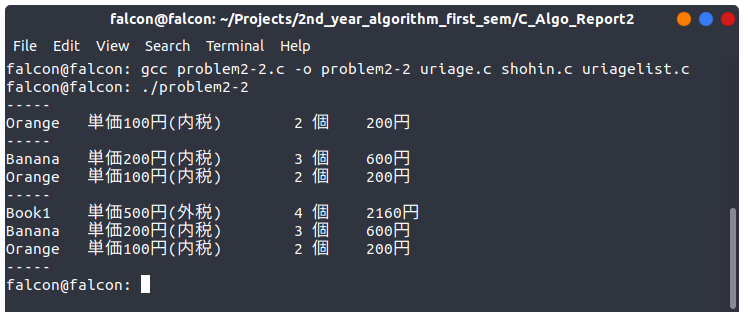
\includegraphics[width=0.8\textwidth]{problem2-2.png}
	\caption{課題2-2実行結果}
\end{figure}

\subsubsection{プログラムの解説}
\begin{itemize}
    \item このプログラムでは課題1で定義した、URIAGE型、SHOHIN型を使っている。
\end{itemize}
関数 newListは引数がなく、返り値がURIAGELIST型の関数である。この関数を呼び出すとmallocを使ってヒープ領域にURIAGELISTの大きさ分のメモリを確保し、メモリアロケーションが成功するとnewNode変数にメモリ上に確保した領域への参照ポインターが格納される。もしアロケーションに失敗するとmalloc関数からNULLが返され、newNodeに格納される。newNodeがNULLの場合はNULLを返す。


\subsection{課題2-3}
\begin{itemize}
    \item 線形リストにおいて、動的に確保したすべてのノードをfree関数により解放す る関数 void freeUriageList(URIAGELIST*l,int purge) を作成しなさい。
\end{itemize}
\subsubsection{uriagelist.h}
\begin{lstlisting}[language=C]
    #ifndef C_ALGO_REPORT2_URIAGELIST_H
    #define C_ALGO_REPORT2_URIAGELIST_H
    
    #endif //C_ALGO_REPORT2_URIAGELIST_H
    
    
    typedef struct uriagelist {
        struct uriagelist* next;
        URIAGE *uriage;
    } URIAGELIST;
    
    void printUriageList(URIAGELIST* l);
    URIAGELIST* newlist(void);
    void freeUriageList (URIAGELIST *l , int purge);
\end{lstlisting}

\subsubsection{uriagelist.c}
\begin{lstlisting}[language=C]
    #include <stdio.h>
    #include <stdlib.h>
    #include "uriage.h"
    #include "shohin.h"
    #include "uriagelist.h"
    
    void printUriageList(URIAGELIST *l) {
        if (l->uriage == NULL) {
            return;
        }
        while (l->next != NULL) {
            // 課題1のuriage.cで定義されているprintUriage関数を使っている。
            printUriage(l->uriage);
            l = l->next;
        }
    }
    
    URIAGELIST *newlist(void) {
        URIAGELIST *newNode = malloc(sizeof(URIAGELIST));
        if (newNode == NULL) {
            return NULL;
        } else {
            newNode->next = NULL;
            newNode->uriage = NULL;
            return newNode;
        }
    }
    
    void freeUriageList(URIAGELIST *l, int purge) {
        while (l->next != NULL) {
            if (purge == 1) {
                free(l->uriage);
            }
            URIAGELIST *previous_l = l;
            l = l->next;
            free(previous_l);
        }
    }
\end{lstlisting}

\subsubsection{テストプログラム2-3}
\begin{lstlisting}[language=C]
    #include <stdio.h>
    #include <stdlib.h>
    #include "shohin.h"
    #include "uriage.h"
    #include "uriagelist.h"
    int main(void){
        URIAGE u1={1,2};
        URIAGE u2={2,3};
        URIAGE u3={3,4};
        URIAGE *up1;
        URIAGE *up2;
        URIAGE *up3;
        URIAGELIST *l0;
        URIAGELIST *l1;
        URIAGELIST *l2;
        URIAGELIST *l3;
        if((l0=newlist())==NULL){
            fprintf(stderr,"領域を確保できませんでした");
            return 2;
        }
        if((l1=newlist())==NULL){
            fprintf(stderr,"領域を確保できませんでした");
            free(l0);
            return 2;
        }
        if((l2=newlist())==NULL){
            fprintf(stderr,"領域を確保できませんでした");
            free(l1);
            free(l0);
            return 2;
        }
        if((l3=newlist())==NULL){
            fprintf(stderr,"領域を確保できませんでした");
            free(l2);
            free(l1);
            free(l0);
            return 2;
        }
        l1->next=l0;
        l1->uriage=&u1;
        l2->next=l1;
        l2->uriage=&u2;
        l3->next=l2;
        l3->uriage=&u3;
        printUriageList(l3);
        printf("-----\n");
        freeUriageList(l3,0);
    
        if((l0=newlist())==NULL){
            fprintf(stderr,"領域を確保できませんでした");
            return 2;
        }
        if((l1=newlist())==NULL){
            fprintf(stderr,"領域を確保できませんでした");
            free(l0);
            return 2;
        }
        if((l2=newlist())==NULL){
            fprintf(stderr,"領域を確保できませんでした");
            free(l1);
            free(l0);
            return 2;
        }
        if((l3=newlist())==NULL){
            fprintf(stderr,"領域を確保できませんでした");
            return 2;
        }
        if((up1=malloc(sizeof(URIAGE)))==NULL){
            fprintf(stderr,"領域を確保できませんでした");
            free(l2);
            free(l1);
            free(l0);
            return 2;
        }
        if((up2=malloc(sizeof(URIAGE)))==NULL){
            fprintf(stderr,"領域を確保できませんでした");
            free(l2);
            free(l1);
            free(l0);
            free(up1);
            return 2;
        }
        if((up3=malloc(sizeof(URIAGE)))==NULL){
            fprintf(stderr,"領域を確保できませんでした");
            free(l2);
            free(l1);
            free(l0);
            free(up2);
            free(up1);
            return 2;
        }
        *up1=u1;
        *up2=u2;
        *up3=u3;
        l1->next=l0;
        l1->uriage=up1;
        l2->next=l1;
        l2->uriage=up2;
        l3->next=l2;
        l3->uriage=up3;
        printUriageList(l3);
        printf("-----\n");
        freeUriageList(l3,1);
        return 0;
    }
\end{lstlisting}

\subsubsection{実行結果}
\begin{figure}[H]
	\centering
	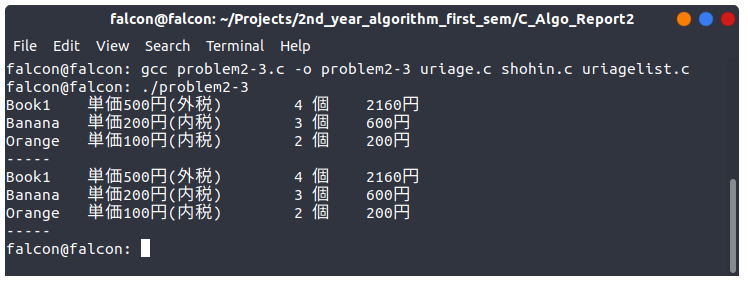
\includegraphics[width=0.8\textwidth]{problem2-3.png}
	\caption{課題2-3実行結果}
\end{figure}

\subsubsection{プログラムの解説}
\begin{itemize}
    \item このプログラムでは課題1で定義した、URIAGE型、SHOHIN型を使っている。
\end{itemize}

freeUriageListはURIAGELIST型のポインター(*l)とint型のpurgeを引数とし、返り値がvoidの関数である。この関数で引数として受け取ったポインター *lはある線形リストの先頭のノードを指していて、この関数を実行すると線形リストのすべてのノードが使っているメモリを開放する。また、この線形リストはデータへの参照ポインターを含む uriageと次のノードのポインターを含むnextで構成されており、引数のpurgeが1の場合は各ノードのuriageポインターが参照しているデータが使ってメモリも開放する。purgeが0の場合はすべてのノードにアロケートされている領域だけを開放する。


\subsection{課題2-4}

\begin{itemize}
    \item URIAGEのポインターを受け取ると、URIAGELIST のノードで作られた線形リス トの先頭に、ノードを追加することで追加する URIAGELIST* add(URIAGELIST* l, URIAGE* u) 関数を作成しなさい。
\end{itemize}
\subsubsection{uriagelist.h}
\begin{lstlisting}[language=C]
    #ifndef C_ALGO_REPORT2_URIAGELIST_H
    #define C_ALGO_REPORT2_URIAGELIST_H
    
    #endif //C_ALGO_REPORT2_URIAGELIST_H
    
    
    typedef struct uriagelist {
        struct uriagelist* next;
        URIAGE *uriage;
    } URIAGELIST;
    
    void printUriageList(URIAGELIST* l);
    URIAGELIST* newlist(void);
    void freeUriageList (URIAGELIST *l , int purge);
    URIAGELIST* add(URIAGELIST* l, URIAGE* u);
\end{lstlisting}

\subsubsection{uriagelist.c}
\begin{lstlisting}[language=C]
    #include <stdio.h>
    #include <stdlib.h>
    #include "uriage.h"
    #include "shohin.h"
    #include "uriagelist.h"
    
    
    void printUriageList(URIAGELIST *l) {
        if (l->uriage == NULL) {
            return;
        }
        while (l->next != NULL) {
            // 課題1のuriage.cで定義されているprintUriage関数を使っている。
            printUriage(l->uriage);
            l = l->next;
        }
    }
    
    URIAGELIST *newlist(void) {
        URIAGELIST *newNode = malloc(sizeof(URIAGELIST));
        if (newNode == NULL) {
            return NULL;
        } else {
            newNode->next = NULL;
            newNode->uriage = NULL;
            return newNode;
        }
    }
    
    void freeUriageList(URIAGELIST *l, int purge) {
        while (l->next != NULL) {
            if (purge == 1) {
                free(l->uriage);
            }
            URIAGELIST *previous_l = l;
            l = l->next;
            free(previous_l);
        }
    }
    
    URIAGELIST* add (URIAGELIST* l, URIAGE *u){
        URIAGELIST *newNode = newlist();
        newNode->uriage = l->uriage;
        newNode->next = l->next;
        l->uriage = u;
        l -> next = newNode;
    }
\end{lstlisting}

\subsubsection{テストプログラム2-4}
\begin{lstlisting}[language=C]
    #include <stdio.h>
    #include <stdlib.h>
    #include "shohin.h"
    #include "uriage.h"
    #include "uriagelist.h"
    int main(void){
        URIAGE u1={1,2};
        URIAGE u2={2,3};
        URIAGE u3={3,4};
        URIAGE* u[]={&u1,&u2,&u3,NULL};
        URIAGE **p;
        URIAGELIST *l;
        URIAGELIST *m;
        if((l=newlist())==NULL){
            fprintf(stderr,"領域を確保できませんでした");
            return 2;
        }
        for(p=u;*p!=NULL;p++){
            if((m=add(l,*p))==NULL){
                fprintf(stderr,"領域を確保できませんでした");
                freeUriageList(l,0);
                return 2;
            }
            printf("追加%s\n", m->uriage==*p?"Ok":"NG");
            printUriageList(l);
            printf("-----\n");
        }
        freeUriageList(l,0);
        return 0;
    }
\end{lstlisting}

\subsubsection{実行結果}
\begin{figure}[H]
	\centering
	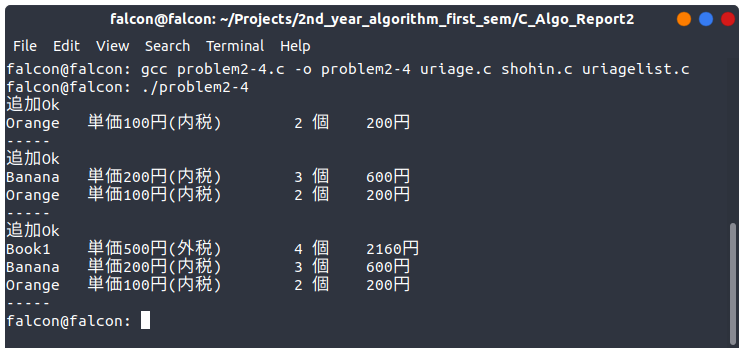
\includegraphics[width=0.8\textwidth]{problem2-4.png}
	\caption{課題2-4実行結果}
\end{figure}

\subsubsection{プログラムの解説}
\begin{itemize}
    \item このプログラムでは課題1で定義した、URIAGE型、SHOHIN型とprintUriage関数を使っている。
\end{itemize}

関数 addはURIAGELIST型のポインター l とURIAGE型のポインター u を引数とし、返り値がURIAGELIST型のポインターである。この関数では最初に、問題2-2で作ったnewlist関数を使ってヒープ領域にメモリをアロケートし、URIAGELIST型の空の線形リストを作る。そして、その線形リストへの参照ポインターをnewNode変数に格納する。次に、その空の線形リストのuriageメンバーに、引数として受け取ったポインター u を格納し、nextには引数として受け取った線形リストの先頭ノードを指しているポインター (*l) を格納する。そして*lのnextをnewNodeへの参照ポインターで置き換える。こうすることでnewNodeが引数*lの線形リストの先頭ノードになる。

\subsection{考察}
今回の課題を解いてレポート書くにあたって、構造体のメンバーに別の構造体のポインターを格納するパラダイムについて理解することできた。また、これを使って線形リストを構成する方法や線形リストの値を参照する方法について理解できた。問2-4では線形リストの削除や順序を変更する方法そして、線形リストの任意のポイントにノードを追加する方法について理解できた。\\
問2-3ではヒーブ領域にメモリをアロケートしたり、アロケートしたメモリを使わなくなったら開放する方法について理解できた。


\end{document}
